% Beamer Presentation and Lecture Note Template
% Version 0.1
% by Paul Vesey

\mode<presentation> {
\usetheme{Antibes}
\setbeamercovered{invisible}
\setbeamertemplate{footline}[frame number]
\setbeamertemplate{navigation symbols}{} 
}

\usepackage{eurosym}
\usepackage{graphicx}
\usepackage{wasysym}
\usepackage{hyperref}
\usepackage{amsmath}
\usepackage{amssymb}
\usepackage{mathtools}
\usepackage{tikz}
\usepackage{pgf}
\usepackage{pgfplots}
\usepackage{pxfonts}
\usepackage{textcomp}
\usepackage{verbatim}
\usepackage{color}
\usepackage{xcolor}
\usepackage{fix-cm}


\author{Paul Vesey}
\institute[TUS]
{
Technological University of the Shannon \\
\medskip
{\emph{paul.vesey@tus.ie}}
}
\date{Autumn 2022}



%\usepackage{bm} 
% For typesetting bold math (not \mathbold)
%\logo{\includegraphics[height=0.6cm]{yourlogo.eps}}
%
\title[Project Management \& BIM]{Introduction to Project Management}


\begin{document}
%
\usetikzlibrary{arrows}
\usepgflibrary{patterns}



\thispagestyle{empty} % Remove page numbering on this page

%----------------------------------------------------------------------------------------
%	TITLE SECTION
%----------------------------------------------------------------------------------------

\hrule

\vspace*{0.7cm} % Space between the start of the title and the top of the grey box


\begin{flushright}
\Huge Project Management \& Building Information Modelling \\
\vspace*{0.7cm}
\Large BSc (Hons) in Construction Management\\
BSc (Hons) in Civil Engineering Management\\
Year 4 (2021-2022)
\end{flushright}

\vspace*{0.7cm} % Space between the end of the title and the bottom of the grey box
	
\normalsize

\hrule

%----------------------------------------------------------------------------------------

\vfill % Space between the title box and author information

%----------------------------------------------------------------------------------------
%	AUTHOR NAME AND INFORMATION SECTION
%----------------------------------------------------------------------------------------

{\centering \large 
\hfill Paul Vesey, \scriptsize BEng (Hons), MIE, HDip\normalsize \\
\hfill Limerick Institute of Technology \\
\hfill Department of the Built Environment \\
\hfill \texttt{https://paulvesey.wordpress.com} \\
\vspace*{0.7cm} 
\hrule} % Horizontal line, thickness changed here

%----------------------------------------------------------------------------------------

\clearpage % Whitespace to the end of the page

\newpage




\thispagestyle{empty}
\tableofcontents
\newpage
\section{Introduction}


\begin{frame}
\titlepage
\end{frame}\begin{center}\line(1,0){250}\end{center}
%
%
\begin{center}\line(1,0){250}\end{center}



\begin{frame}
\frametitle{What is a Project?}
A project is a temporary endeavour to create a unique product, service or result.\\
\begin{itemize}
\item Temporary: it has a start and an end
\item Unique Product, Service or Result
\item Progressive Elaboration
\end{itemize}
\end{frame}
\begin{center}\line(1,0){250}\end{center}





\section{Value Delivery}

\section{Creating Value}

\begin{frame}
\frametitle{Creating Value}
 \begin{figure}
    \centering
        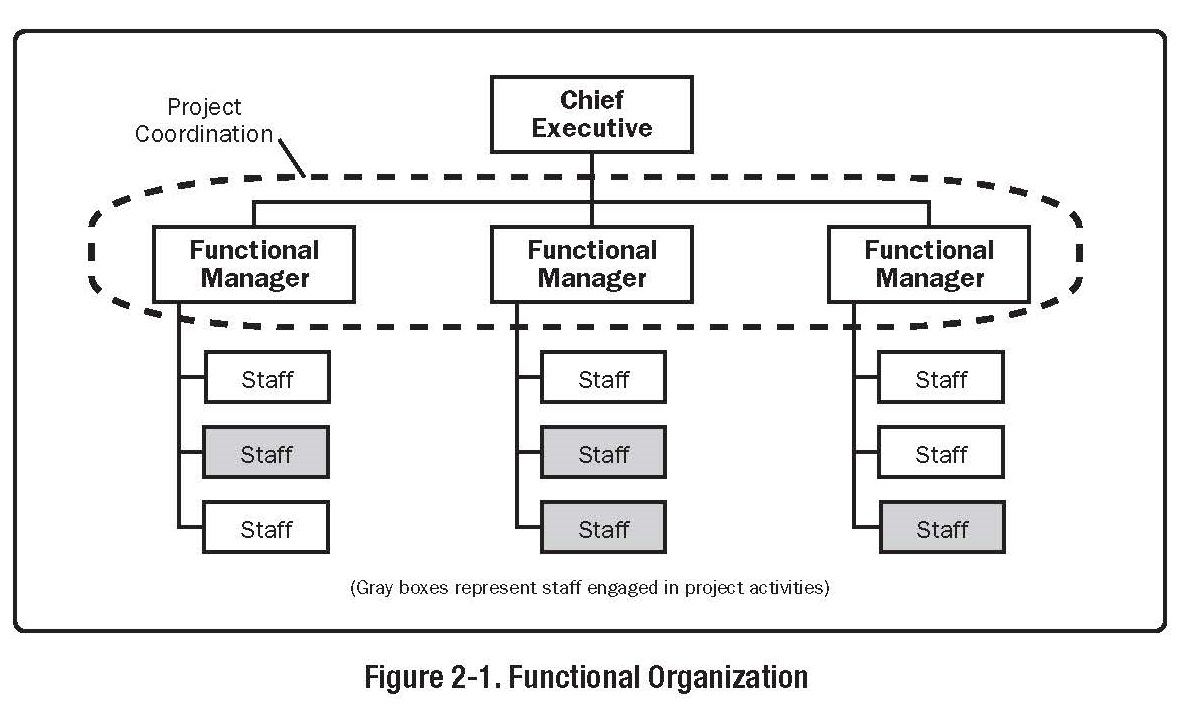
\includegraphics[width = 8cm]{../images/standard/Fig2-1.jpg}
    \label{standardfig:2-1}
 \end{figure}
\end{frame}
\begin{center}\line(1,0){250}\end{center}


\begin{frame}
\frametitle{Project ????}
 \begin{figure}
    \centering
        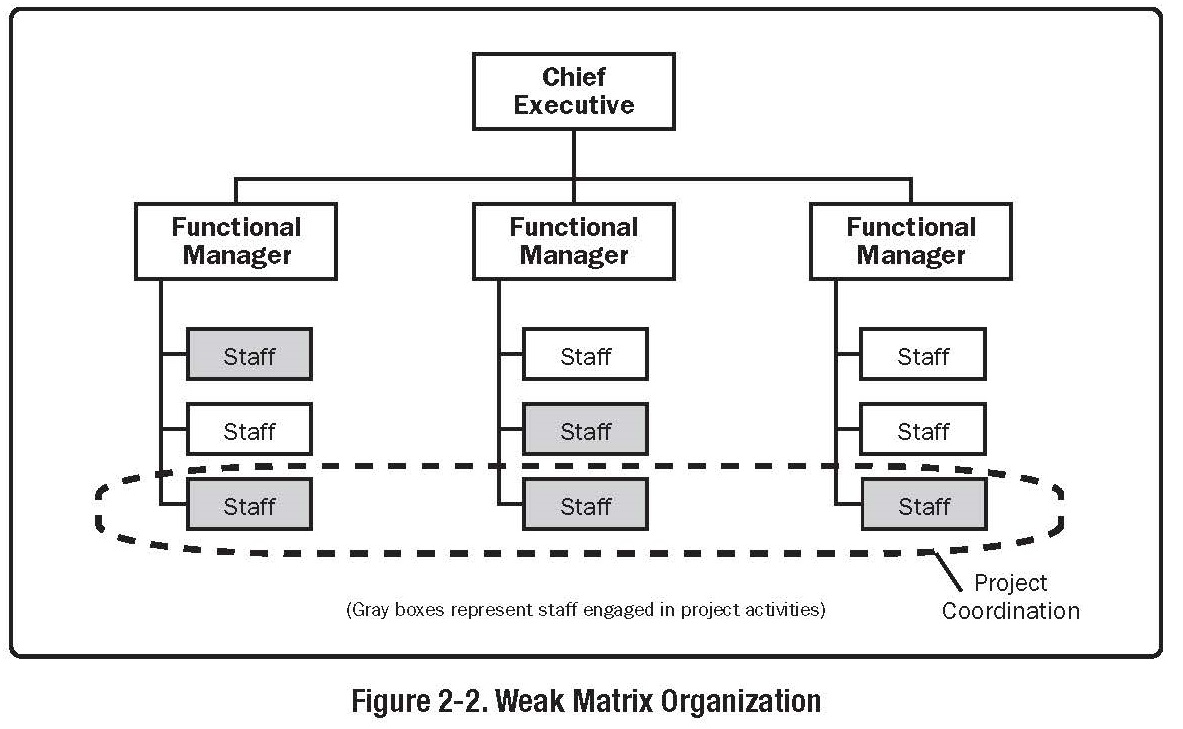
\includegraphics[width = 8cm]{../images/standard/Fig2-2.jpg}
    \label{standardfig:2-2}
 \end{figure}
\end{frame}
\begin{center}\line(1,0){250}\end{center}






\begin{frame}
\frametitle{Project ????}
 \begin{figure}
    \centering
        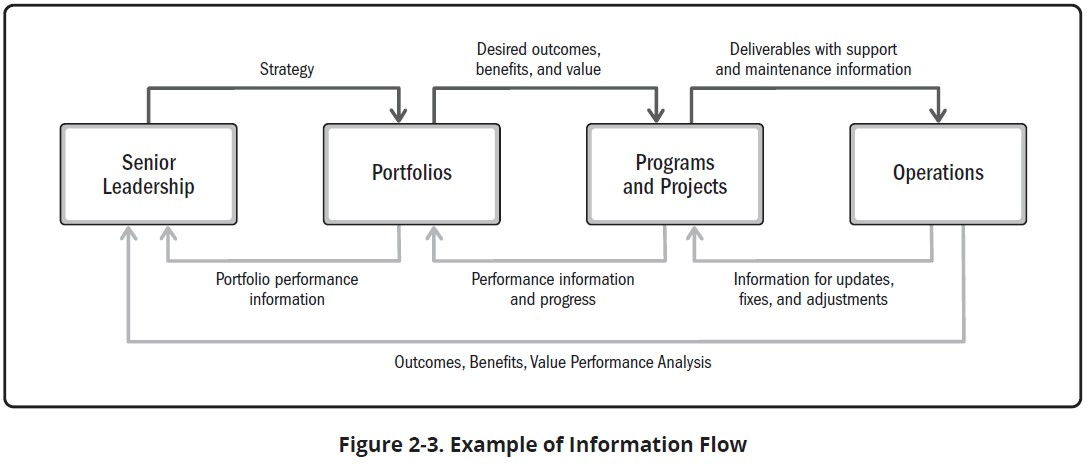
\includegraphics[width = 8cm]{../images/standard/Fig2-3.jpg}
    \label{standardfig:2-3}
 \end{figure}
\end{frame}
\begin{center}\line(1,0){250}\end{center}



\section{Project Management Considerations}


\begin{frame}
\frametitle{Project Management Considerations}
 \begin{figure}
    \centering
        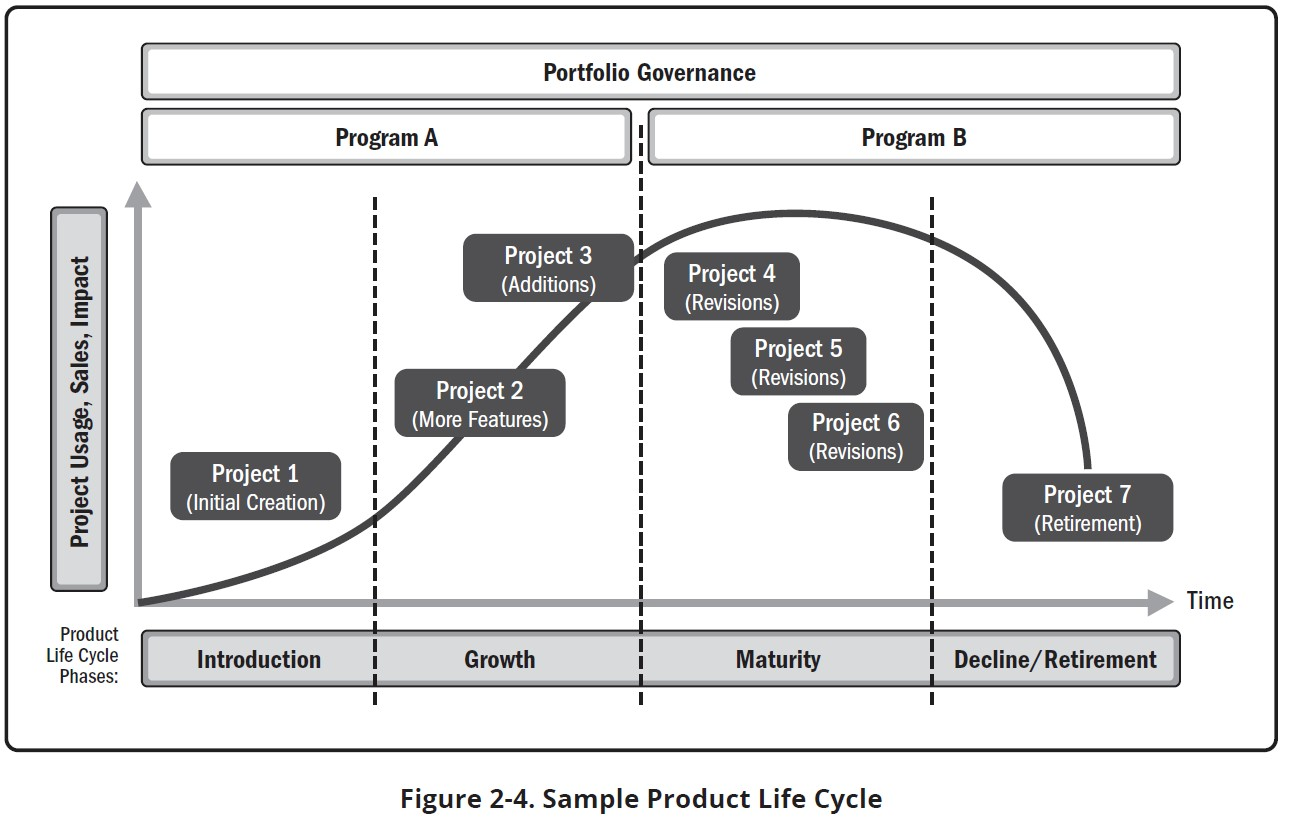
\includegraphics[width = 8cm]{../images/standard/Fig2-4.jpg}
    \label{standardfig:2-4}
 \end{figure}
\end{frame}
\begin{center}\line(1,0){250}\end{center}



\section{Project Management Principles}



\begin{frame}
\frametitle{Project Management Principles}
 \begin{figure}
    \centering
        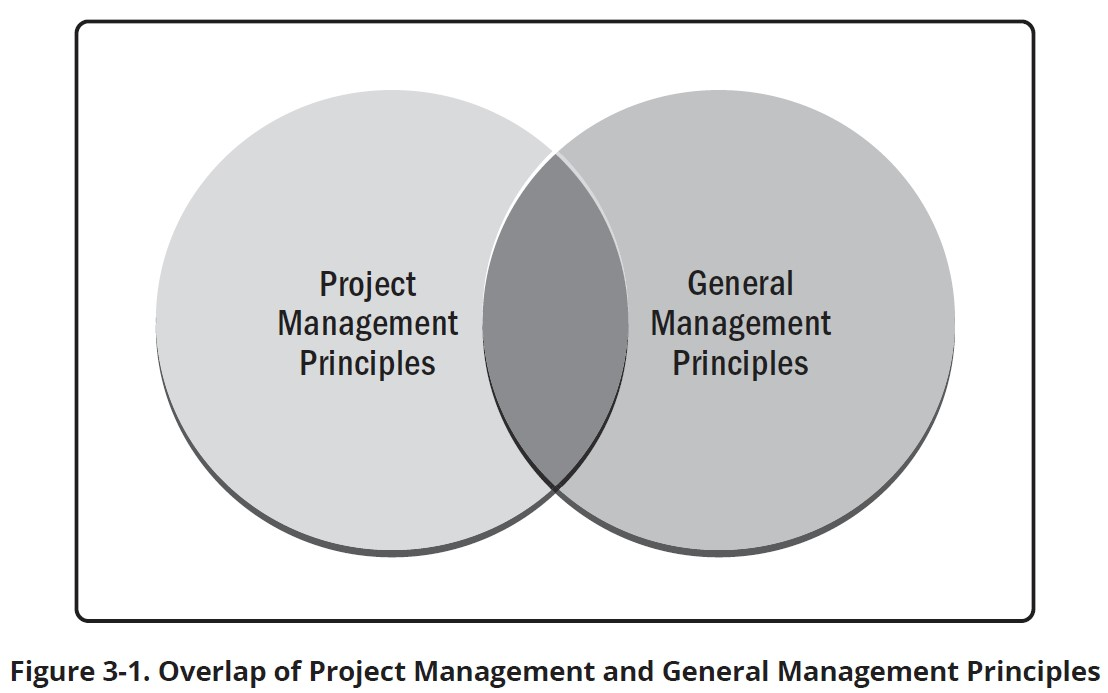
\includegraphics[width = 8cm]{../images/standard/Fig3-1.jpg}
    \label{standardfig:3-1}
 \end{figure}
\end{frame}
\begin{center}\line(1,0){250}\end{center}




\section{Be a Diligent, Respectful, and Caring Steward}


\begin{frame}
\frametitle{Be a Diligent, Respectful, and Caring Steward}
 \begin{figure}
    \centering
        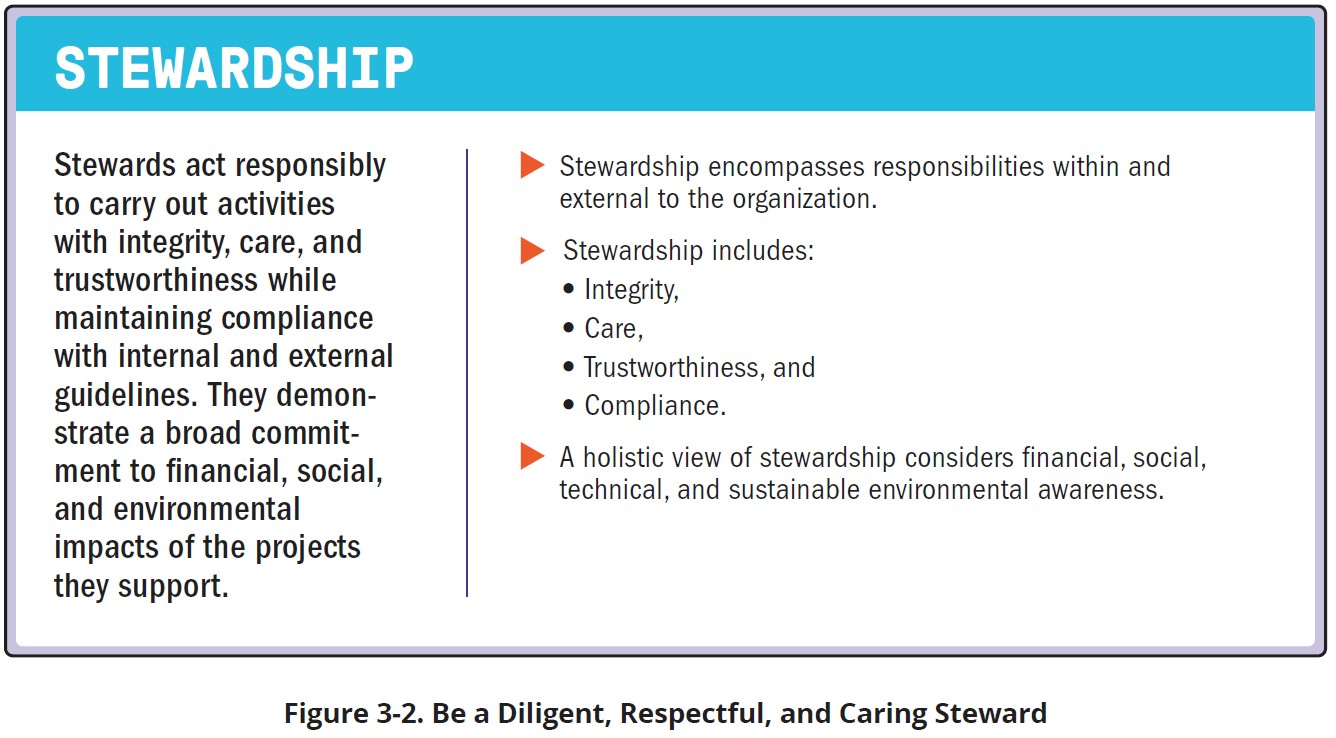
\includegraphics[width = 8cm]{../images/standard/Fig3-2.jpg}
    \label{standardfig:3-2}
 \end{figure}
\end{frame}
\begin{center}\line(1,0){250}\end{center}



\section{Create a Collaborative Team Environment}


\begin{frame}
\frametitle{Create a Collaborative Team Environment}
 \begin{figure}
    \centering
        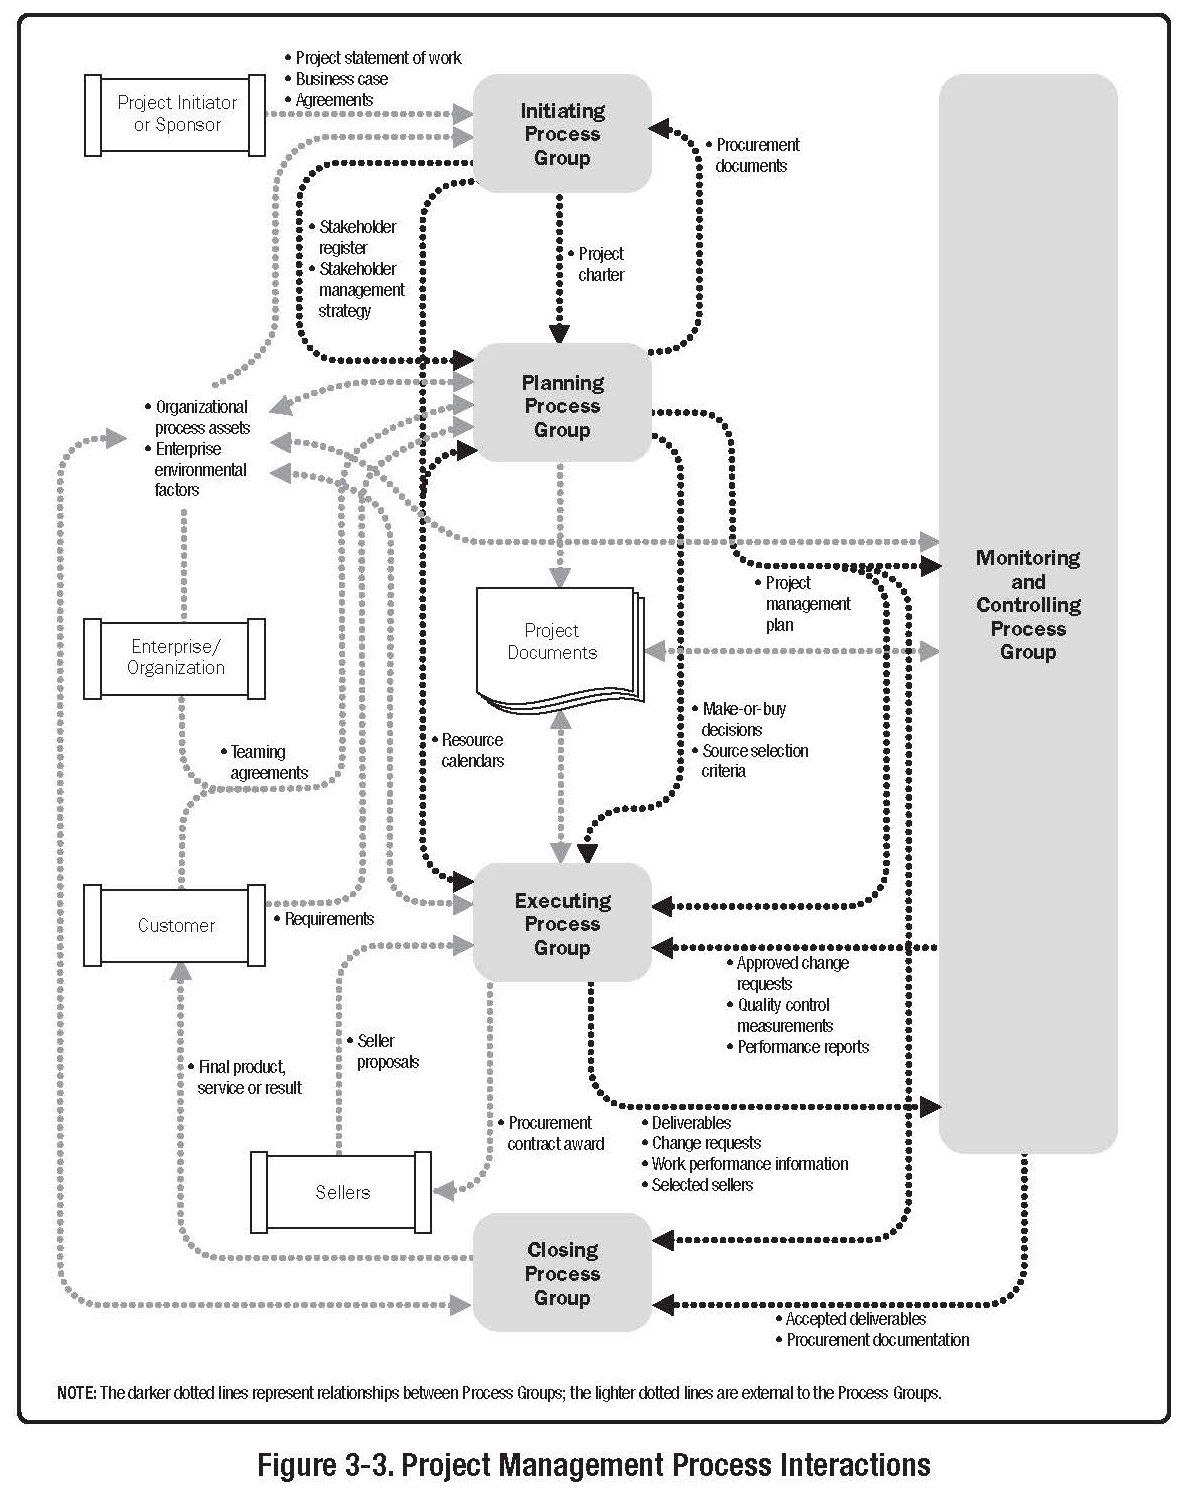
\includegraphics[width = 8cm]{../images/standard/Fig3-3.jpg}
    \label{standardfig:3-3}
 \end{figure}
\end{frame}
\begin{center}\line(1,0){250}\end{center}


\section{Effectively Engage with Stakeholders}


\begin{frame}
\frametitle{Effectively Engage with Stakeholders}
 \begin{figure}
    \centering
        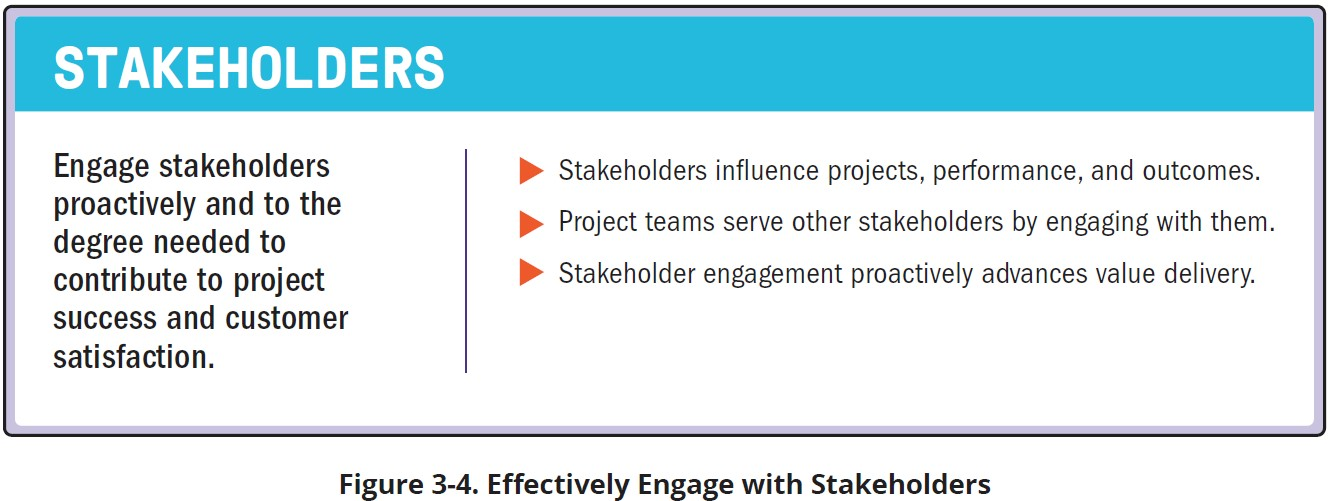
\includegraphics[width = 8cm]{../images/standard/Fig3-4.jpg}
    \label{standardfig:3-4}
 \end{figure}
\end{frame}
\begin{center}\line(1,0){250}\end{center}



\section{Focus on Value}


\begin{frame}
\frametitle{Focus on Value}
 \begin{figure}
    \centering
        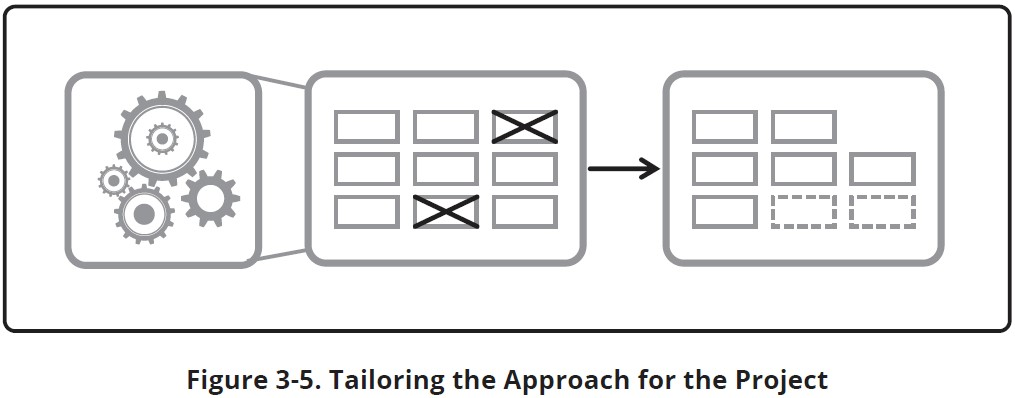
\includegraphics[width = 8cm]{../images/standard/Fig3-5.jpg}
    \label{standardfig:3-5}
 \end{figure}
\end{frame}
\begin{center}\line(1,0){250}\end{center}



\section{Recognise, Evaluate, and Respond to System Interactions}

\begin{frame}
\frametitle{Recognise, Evaluate, and Respond to System Interactions}
 \begin{figure}
    \centering
        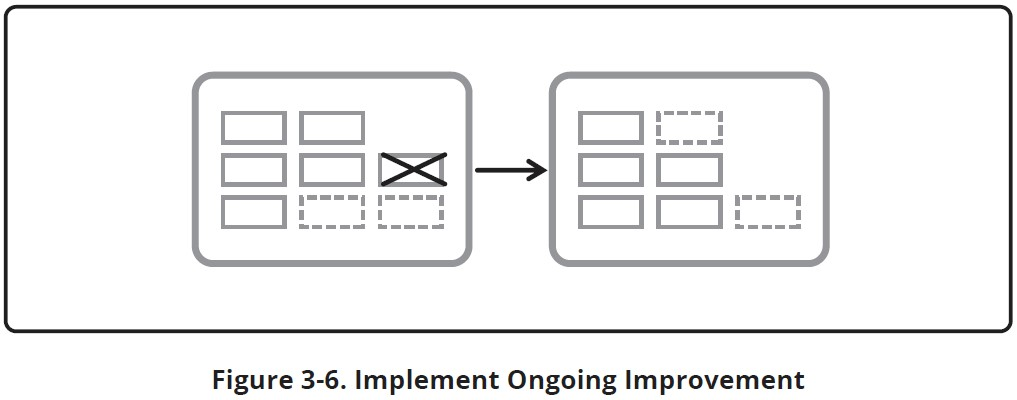
\includegraphics[width = 8cm]{../images/standard/Fig3-6.jpg}
    \label{standardfig:3-6}
 \end{figure}
\end{frame}
\begin{center}\line(1,0){250}\end{center}



\section{Demonstrate Leadership Behaviors}


\begin{frame}
\frametitle{Demonstrate Leadership Behaviors}
 \begin{figure}
    \centering
        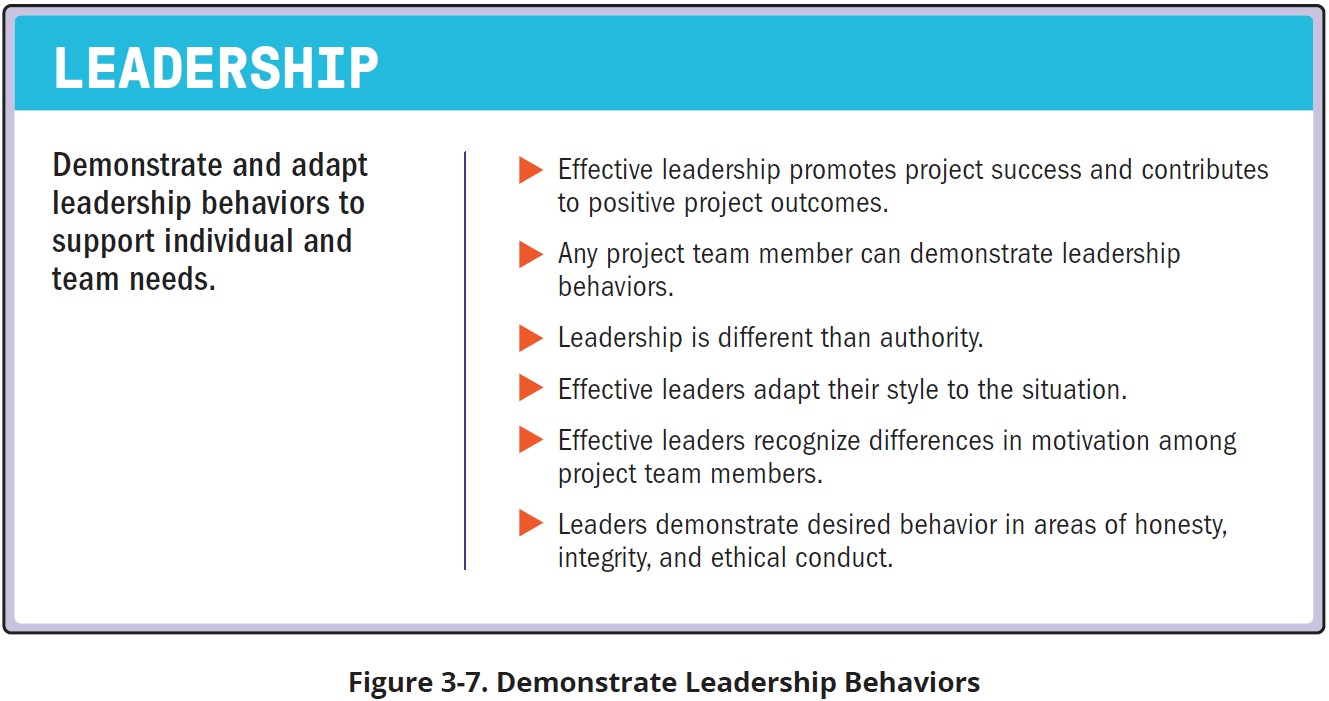
\includegraphics[width = 8cm]{../images/standard/Fig3-7.jpg}
    \label{standardfig:3-7}
 \end{figure}
\end{frame}
\begin{center}\line(1,0){250}\end{center}



\section{Tailor Based on Context}


\begin{frame}
\frametitle{Tailor Based on Context}
 \begin{figure}
    \centering
        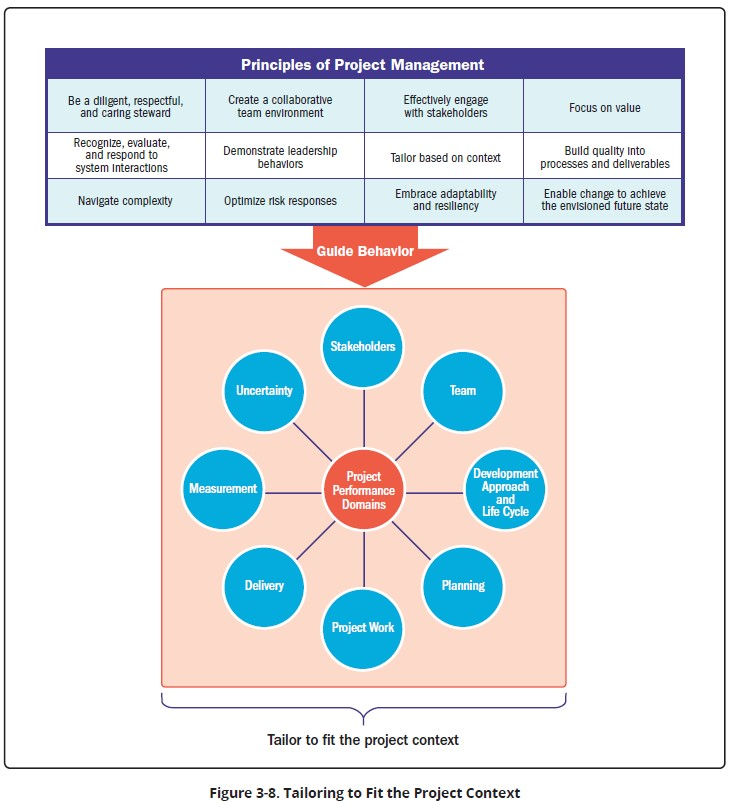
\includegraphics[width = 8cm]{../images/standard/Fig3-8.jpg}
    \label{standardfig:3-8}
 \end{figure}
\end{frame}
\begin{center}\line(1,0){250}\end{center}




\section{Build Quality into Processes and Deliverables}



\begin{frame}
\frametitle{Build Quality into Processes and Deliverables}
 \begin{figure}
    \centering
        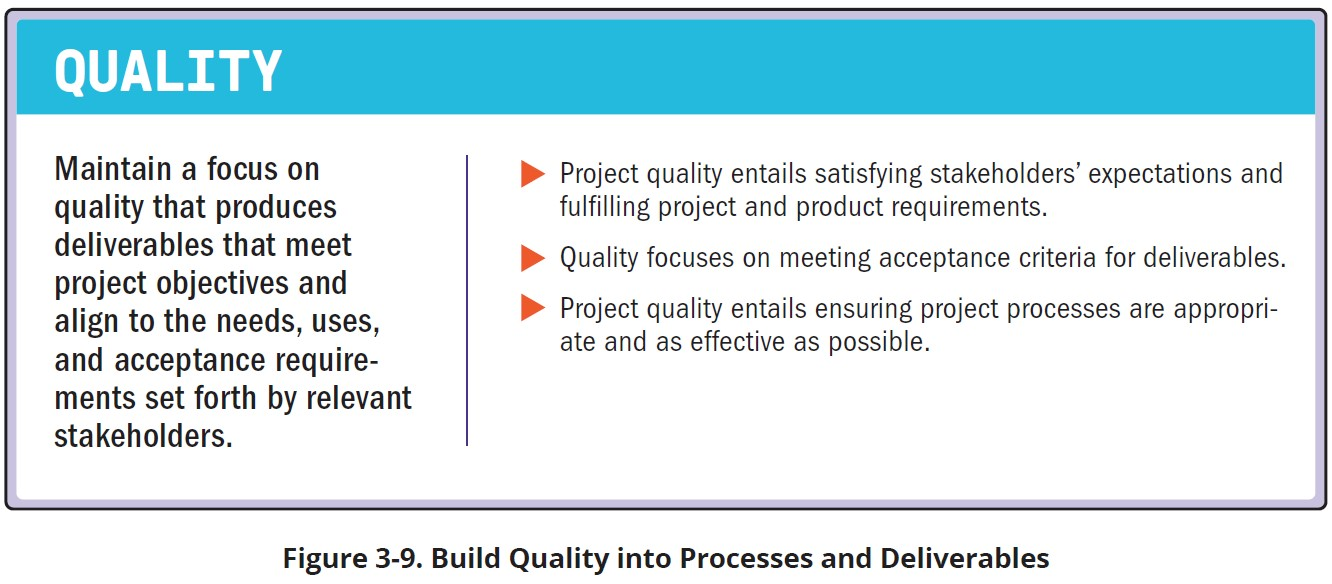
\includegraphics[width = 8cm]{../images/standard/Fig3-9.jpg}
    \label{standardfig:3-9}
 \end{figure}
\end{frame}
\begin{center}\line(1,0){250}\end{center}



\section{Navigate Complexity}


\begin{frame}
\frametitle{Navigate Complexity}
 \begin{figure}
    \centering
        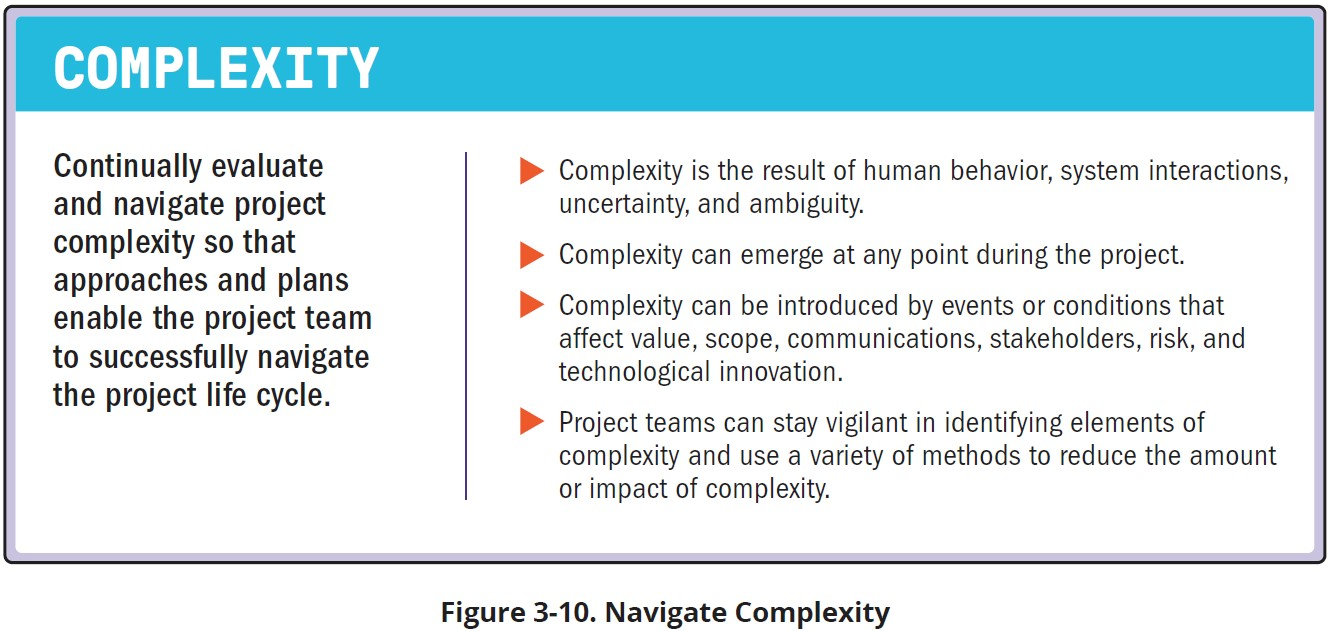
\includegraphics[width = 8cm]{../images/standard/Fig3-10.jpg}
    \label{standardfig:3-10}
 \end{figure}
\end{frame}
\begin{center}\line(1,0){250}\end{center}



\section{Optimize Risk Responses}

\begin{frame}
\frametitle{Optimize Risk Responses}
 \begin{figure}
    \centering
        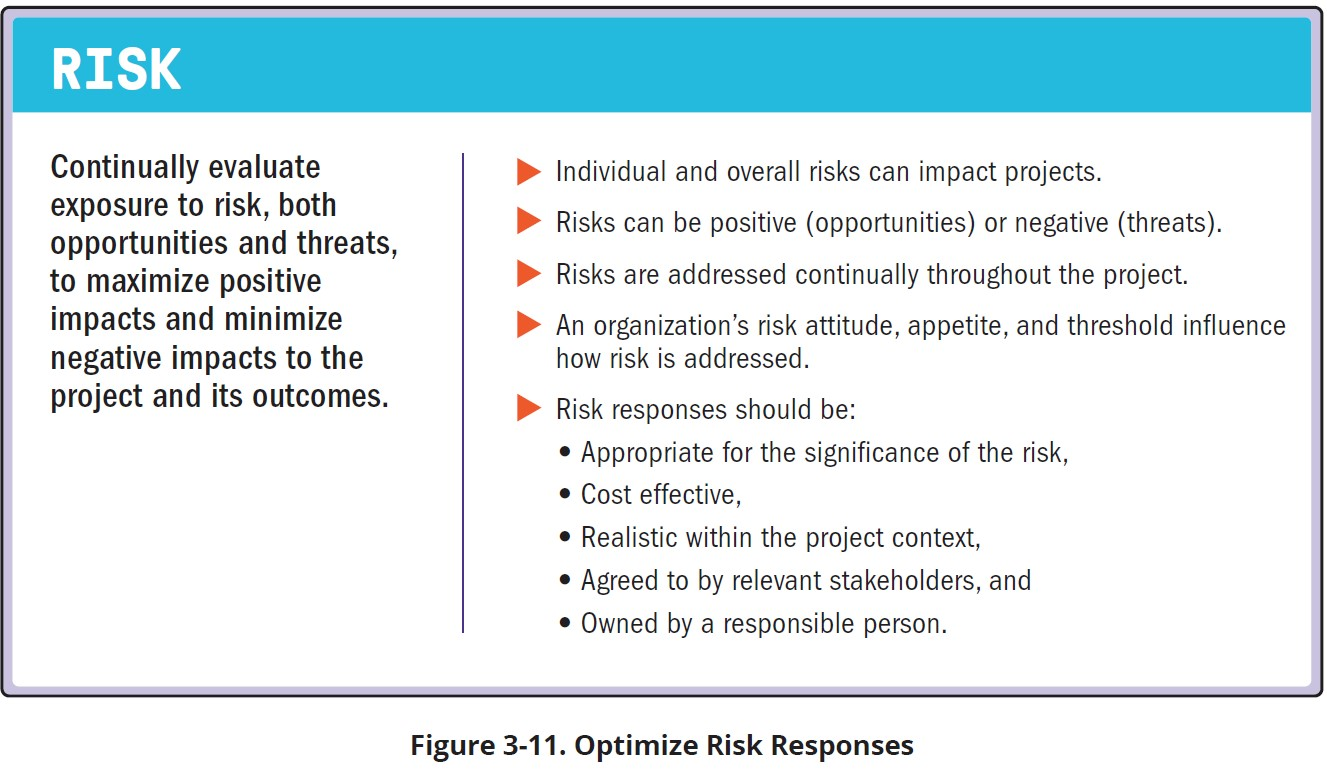
\includegraphics[width = 8cm]{../images/standard/Fig3-11.jpg}
    \label{standardfig:3-11}
 \end{figure}
\end{frame}
\begin{center}\line(1,0){250}\end{center}



\section{Embrace Adaptability and Resiliency}

\begin{frame}
\frametitle{Embrace Adaptability and Resiliency}
 \begin{figure}
    \centering
        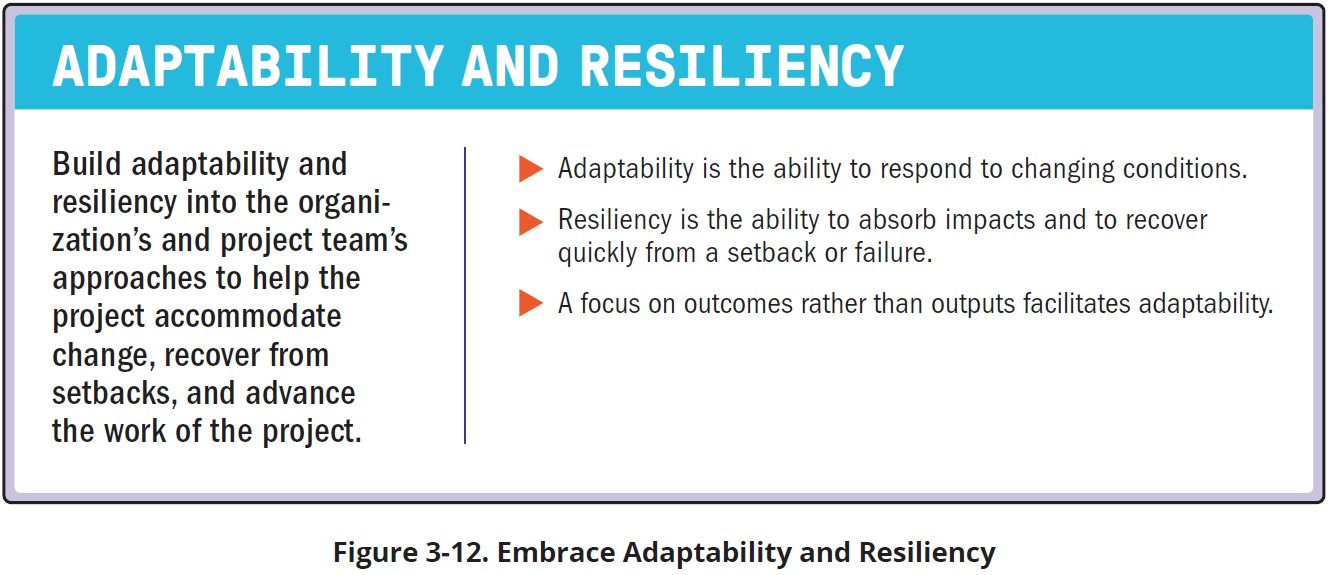
\includegraphics[width = 8cm]{../images/standard/Fig3-12.jpg}
    \label{standardfig:3-12}
 \end{figure}
\end{frame}
\begin{center}\line(1,0){250}\end{center}



\section{Enable Change to Achieve the Envisioned Future State}

\begin{frame}
\frametitle{Enable Change to Achieve the Envisioned Future State}
 \begin{figure}
    \centering
        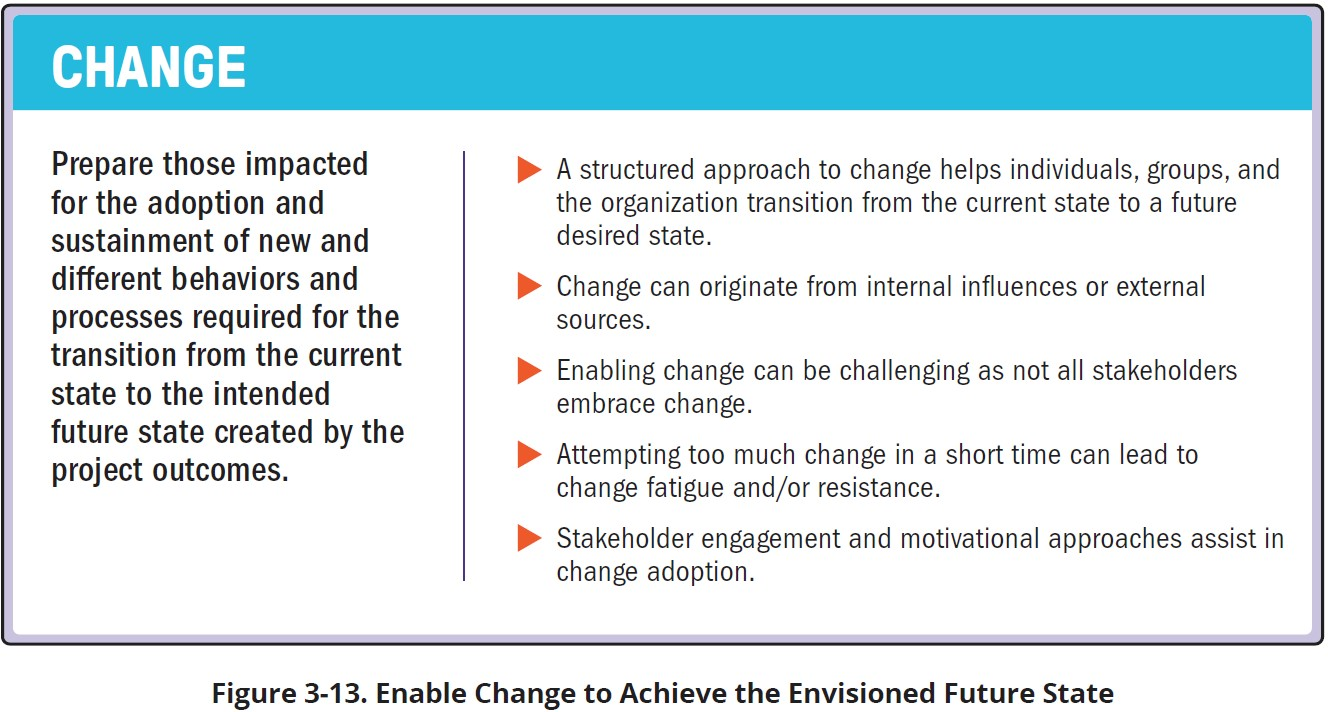
\includegraphics[width = 8cm]{../images/standard/Fig3-13.jpg}
    \label{standardfig:3-13}
 \end{figure}
\end{frame}
\begin{center}\line(1,0){250}\end{center}




\end{document}
